\documentclass{article}

% Packages for code listing and syntax highlighting
\usepackage{listings}
\usepackage{xcolor}
\usepackage[margin=3cm]{geometry} % Adjust the margin value as desired
\usepackage{setspace}
\usepackage{tikz}
\usepackage{graphicx}
\usepackage{float}
\usepackage{textcomp}
\usepackage{multicol}
\usepackage{enumitem}

\onehalfspacing

% Define the color theme
\definecolor{codebackground}{RGB}{242, 242, 242}
\definecolor{codekeyword}{RGB}{0, 0, 255}
\definecolor{codecomment}{RGB}{63, 127, 95}
\definecolor{codestring}{RGB}{163, 21, 21}

% Code listing style for all languages
\lstdefinestyle{mystyle}{
    backgroundcolor=\color{codebackground},
    basicstyle=\footnotesize\ttfamily,
    keywordstyle=\color{codekeyword}\bfseries,
    commentstyle=\color{codecomment}\itshape,
    stringstyle=\color{codestring},
    numbers=left,
    numberstyle=\tiny\color{codecomment},
    stepnumber=1,
    numbersep=8pt,
    showstringspaces=false,
    breaklines=true,
    frame=single,
    frameround=none,
    framesep=5pt,
    rulecolor=\color{codebackground},
    tabsize=4,
    captionpos=b,
    xleftmargin=15pt,
    xrightmargin=15pt
}

% Set the default style for code listings
\lstset{style=mystyle}

% Additional packages and settings for math typesetting
\usepackage{amsmath}
\usepackage{amssymb}
\usepackage{bm}

% Define your document content
\begin{document}

\title{Memory, Storing Data, and Indirection}
\author{Abyan Majid}
\date{July 7, 2023}
\maketitle

\section{Memory}
Below is the basic structure of a memory chip.
\begin{center}
    \begin{tabular}{@{}c|c|}
        \multicolumn{1}{@{}c}{\textbf{Address}} & \multicolumn{1}{c@{}}{\textbf{Cell}} \\
        \cline{2-2}
        $0$ & Data 0 \\
        \cline{2-2}
        $1$ & Data 1 \\
        \cline{2-2}
        $2$ & Data 2 \\
        \cline{2-2}
        $3$ & Data 3 \\
        \cline{2-2}
        ... & ... \\
        \cline{2-2}
        $n-1$ & Data $n-1$ \\
        \cline{2-2}
    \end{tabular}

    \vspace{0.25cm}

    \hspace{1.5cm}
    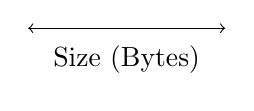
\begin{tikzpicture}
    \draw[<->] (0,-0.5) -- (2.5,-0.5);
    \node at (1.25,-0.9) {Size (Bytes)};
    \end{tikzpicture}
\end{center}

\noindent A memory chip is comprised of memory cells. Each memory cell:
\begin{itemize}
    \item is capable of storing data of a specified size in bytes.
    \item has a unique address that points to it.
\end{itemize}

\noindent When a memory is first initialized, it has "garbage" - that is, it has random or unpredictable data. "Garbage" therefore may be remnants of data from previous programs, uninitialized variables, and many more possibilities.

\subsection{Memory size \& byte conversion}

To compute the size of a memory, you multiply the number of cells with the size of the cells.
$$\text{Memory size = No. of Cells}\times\text{Cell Size}$$

\noindent All cells in a memory always have the same size. However, the size itself depends on the memory chip, hence may differ compared to other memory chips. Some memory chips have cells each sized 1 byte, some others 2 byte, 3, 4, etc.

\vspace{0.5cm}

\noindent Below lists the bit-to-byte and to higher units conversions:

\begin{itemize}
    \item 8 Bits $\rightarrow$ 1 Byte
    \item 1024 Bytes $\rightarrow$ 1 Kilobyte ($2^{10}$ bytes)
    \item 1024 Kilobytes $\rightarrow$ 1 Megabyte ($2^{20}$ bytes)
    \item 1024 Megabytes $\rightarrow$ 1 Gigabyte ($2^{30}$ bytes)
    \item 1024 Gigabyte $\rightarrow$ 1 Terabyte ($2^{40}$ bytes)
    \item 1024 Terabyte $\rightarrow$ 1 Petabyte ($2^{50}$ bytes)
    \item 1024 Petabyte $\rightarrow$ 1 Exabyte ($2^{60}$ bytes)
\end{itemize}
\noindent and so on...

\subsection{Operations with memory}
There's two operations you can do with a memory:
\begin{itemize}
    \item Write (arg=address, data): What it means to "write" is simply to store data in a memory cell/s. When you do a "write" operation, you usually pass two arguments (1) the address of the cell, and (2) the data to be stored.
    \item Read (arg=address): What it means to "read" is to simply know or see the data stored in a memory cell. When you do a "read" operation, you simply pass the address of the cell which contains the data you wish to read.
\end{itemize}

\section{Storing data in memory}

\subsection{Storing data of the same size as the cells'}

Suppose we have a memory chip with cells sized 1 byte each.

\begin{center}
    \begin{tabular}{@{}c|c|}
        \multicolumn{1}{@{}c}{\textbf{Address}} & \multicolumn{1}{c@{}}{\textbf{Cell}} \\
        \cline{2-2}
        ... & ... \\
        \cline{2-2}
        253 &  \\
        \cline{2-2}
        254 &  \\
        \cline{2-2}
        255 &  \\
        \cline{2-2}
        256 &  \\
        \cline{2-2}
        ... & ... \\
        \cline{2-2}
    \end{tabular}

    \vspace{0.25cm}

    \hspace{1.5cm}
    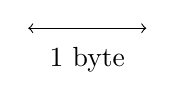
\begin{tikzpicture}
    \draw[<->] (0,-0.5) -- (1.5,-0.5);
    \node at (0.75,-0.9) {1 byte};
    \end{tikzpicture}
\end{center}

\noindent And we wanna store an integer 158 to the 254th cell. If you do the math, the binary representation of the integer 158 is \underline{0b10011110}. You should notice that 0b10011110 is an 8-bit binary. Since each cell is sized 1 byte = 8 bits, 0b10011110 can be stored into one cell using a write operation (i.e. write(adr=254, data=158), NOTE that this is not actual code, just a visualization.).

\begin{center}
    \begin{tabular}{@{}c|c|}
        \multicolumn{1}{@{}c}{\textbf{Address}} & \multicolumn{1}{c@{}}{\textbf{Cell}} \\
        \cline{2-2}
        ... & ... \\
        \cline{2-2}
        253 &  \\
        \cline{2-2}
        254 & 0b10011110 \\
        \cline{2-2}
        255 &  \\
        \cline{2-2}
        256 &  \\
        \cline{2-2}
        ... & ... \\
        \cline{2-2}
    \end{tabular}

    \vspace{0.25cm}

    \hspace{1.5cm}
    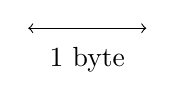
\begin{tikzpicture}
    \draw[<->] (0,-0.5) -- (1.5,-0.5);
    \node at (0.75,-0.9) {1 byte};
    \end{tikzpicture}
\end{center}

\noindent Now that is pretty lengthy, and I hope you realize that even greater data will result in much longer binaries. That's why it is conventional to \underline{\textbf{represent data stored in memory cells in hexadecimal notation}}. If you do the math, the hexadecimal representation of 158 is 9E.

\begin{center}
    \begin{tabular}{@{}c|c|}
        \multicolumn{1}{@{}c}{\textbf{Address}} & \multicolumn{1}{c@{}}{\textbf{Cell}} \\
        \cline{2-2}
        ... & ... \\
        \cline{2-2}
        253 &  \\
        \cline{2-2}
        254 & 0x9E \\
        \cline{2-2}
        255 &  \\
        \cline{2-2}
        256 &  \\
        \cline{2-2}
        ... & ... \\
        \cline{2-2}
    \end{tabular}

    \vspace{0.25cm}

    \hspace{1.5cm}
    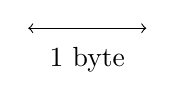
\begin{tikzpicture}
    \draw[<->] (0,-0.5) -- (1.5,-0.5);
    \node at (0.75,-0.9) {1 byte};
    \end{tikzpicture}
\end{center}

\begin{center}
    That looks much neater!
\end{center}

\subsection{Storing data of higher sizes}

Now what if we have a memory cell with cells sized 1 byte each, but we want to store a data that has a size higher than 1 byte?


\begin{center}
    \begin{tabular}{@{}c|c|}
        \multicolumn{1}{@{}c}{\textbf{Address}} & \multicolumn{1}{c@{}}{\textbf{Cell}} \\
        \cline{2-2}
        0 &  \\
        \cline{2-2}
        1 &  \\
        \cline{2-2}
        2 &  \\
        \cline{2-2}
        3 &  \\
        \cline{2-2}
        4 &  \\
        \cline{2-2}
        ... & ... \\
        \cline{2-2}
    \end{tabular}

    \vspace{0.25cm}

    \hspace{1.5cm}
    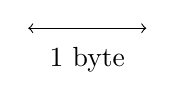
\begin{tikzpicture}
    \draw[<->] (0,-0.5) -- (1.5,-0.5);
    \node at (0.75,-0.9) {1 byte};
    \end{tikzpicture}
\end{center}

\noindent Suppose that we want to store the string "Johan". In ASCII encoding, we have:
\begin{center}
    \begin{tabular}{|c|c|c|}
        \hline
        Character & Hexadecimal & Binary \\
        \hline
        J & 4A & 01001010 \\
        o & 6F & 01101111 \\
        h & 68 & 01101000 \\
        a & 61 & 01100001 \\
        n & 6E & 01101110 \\
        \hline
    \end{tabular}    
\end{center}

\noindent As you can see, in ASCII encoding, each character is exactly 1 byte long. So, even though we can't store "Johan" as a string in one cell, we can store each character in different cells such that when 5 cells are put together, it would read "Johan"!

\begin{center}
    Here's one way to do it:
\end{center}
\begin{center}
    \begin{tabular}{@{}c|c|}
        \multicolumn{1}{@{}c}{\textbf{Address}} & \multicolumn{1}{c@{}}{\textbf{Cell}} \\
        \cline{2-2}
        0 &  0x6F \\
        \cline{2-2}
        1 &  0x6E \\
        \cline{2-2}
        2 &  0x4A \\
        \cline{2-2}
        3 &  0x68\\
        \cline{2-2}
        4 &  0x61 \\
        \cline{2-2}
        ... & ... \\
        \cline{2-2}
    \end{tabular}

    \vspace{0.25cm}

    \hspace{1.5cm}
    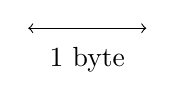
\begin{tikzpicture}
    \draw[<->] (0,-0.5) -- (1.5,-0.5);
    \node at (0.75,-0.9) {1 byte};
    \end{tikzpicture}
\end{center}

\subsection{Endians}
\noindent You may notice that something's amiss. Which is that reading these cells in order, we get "onJha" instead of "Johan". Thing is, that is perfectly valid! You see, what's happening here is we have an \textbf{endian}. An endian is a ordering of multi-byte data in the memory either from the largest to the smallest, or from the smallest to the largest. In this case, our string "Johan" is stored from largest to smallest! If it were to be stored from smallest to largest, we would have the following instead:

\begin{center}
    \begin{tabular}{@{}c|c|}
        \multicolumn{1}{@{}c}{\textbf{Address}} & \multicolumn{1}{c@{}}{\textbf{Cell}} \\
        \cline{2-2}
        0 &  0x61 \\
        \cline{2-2}
        1 &  0x68 \\
        \cline{2-2}
        2 &  0x4A \\
        \cline{2-2}
        3 &  0x6E\\
        \cline{2-2}
        4 &  0x6F \\
        \cline{2-2}
        ... & ... \\
        \cline{2-2}
    \end{tabular}

    \vspace{0.25cm}

    \hspace{1.5cm}
    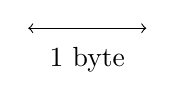
\begin{tikzpicture}
    \draw[<->] (0,-0.5) -- (1.5,-0.5);
    \node at (0.75,-0.9) {1 byte};
    \end{tikzpicture}
\end{center}

\begin{center}
    Both orders are perfectly valid!
\end{center}

\section{Indirection}
Memory indirection is when instead of storing a data to a memory cell, you store a reference that points to another cell. For example, look at the Rust code below.

\begin{lstlisting}[language=Python, caption={Example Python Code}]
    fn main() {
        let x = 42;
        let y = &x;
    }
\end{lstlisting}

\noindent Above is a memory indirection done in Rust, wherein we stored an integer "42" (0x2A in hexadecimal) in the memory, and stored a reference "\&x" in another memory cell - such that if we read the content of $y$, we will get the value of $x$. In our usual memory diagram, the memory indirection may be depicted as follows:

\begin{center}
    \begin{tabular}{@{}c|c|}
        \multicolumn{1}{@{}c}{\textbf{Address}} & \multicolumn{1}{c@{}}{\textbf{Cell}} \\
        \cline{2-2}
        ... & ... \\
        \cline{2-2}
        668 &  0x2A \\
        \cline{2-2}
        669 &   \\
        \cline{2-2}
        700 &   \\
        \cline{2-2}
        701 &  668 \\
        \cline{2-2}
        ... & ... \\
        \cline{2-2}
    \end{tabular}

    \vspace{-3cm}
    \hspace{2.75cm}
    \begin{tikzpicture}[overlay,remember picture]
        \draw[->, bend right=45, thick] (0, -2.25) to[out=0, in=-90] (0, -0.6);
    \end{tikzpicture}
\end{center}

\vspace{3cm}
\noindent In a nutshell, if you store a memory indirection to a cell $B$, which points to the cell $A$, if you read $B$, you will be returned the data stored in $A$.

\end{document}